\documentclass[../../main.tex]{subfiles}
\begin{document}

\begin{flushright}
\footnotesize\textit{【自動文字起こし・要確認】}
\end{flushright}

下の図は線分ABの投影図であり，その各部の寸法は図の通りである．

\begin{figure}[htb]
\centering
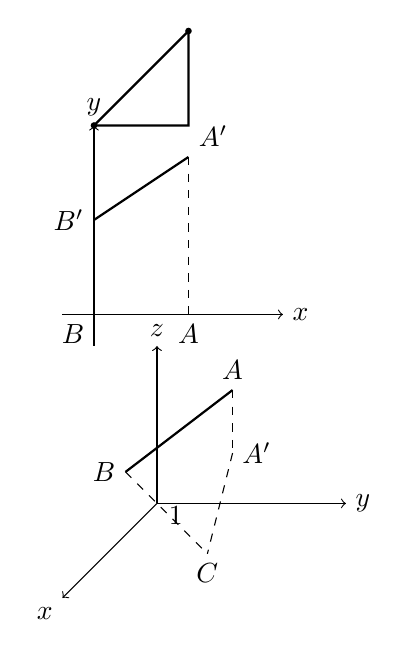
\begin{tikzpicture}[scale=0.8]
  % Projection 1 (Triangle)
  \draw[thick] (0,3) -- (1.5,3) -- (1.5,4.5) -- cycle;
  \draw[dashed] (0,3) -- (1.5,3);
  \fill (0,3) circle (1.5pt);
  \fill (1.5,4.5) circle (1.5pt);
  
  % Projection 2 (2D Axes)
  \begin{scope}[shift={(0,0)}]
    \draw[->] (-0.5,0) -- (3,0) node[right] {$x$};
    \draw[->] (0,-0.5) -- (0,3) node[above] {$y$};
    \draw[thick] (0,1.5) node[left] {$B'$} -- (1.5,2.5) node[above right] {$A'$};
    \draw[dashed] (1.5,2.5) -- (1.5,0) node[below] {$A$};
    \draw[dashed] (0,1.5) -- (0,0);
    \node[below left] at (0,0) {$B$};
  \end{scope}

  % Projection 3 (3D Axes)
  \begin{scope}[shift={(1,-3)}]
    \draw[->] (0,0) -- (3,0) node[right] {$y$};
    \draw[->] (0,0) -- (0,2.5) node[above] {$z$};
    \draw[->] (0,0) -- (-1.5,-1.5) node[below left] {$x$};
    \draw[thick] (-0.5,0.5) node[left] {$B$} -- (1.2,1.8) node[above] {$A$};
    \draw[dashed] (1.2,1.8) -- (1.2,0.8) node[right] {$A'$};
    \draw[dashed] (-0.5,0.5) -- (0.8,-0.8) node[below] {$C$};
    \draw[dashed] (1.2,0.8) -- (0.8,-0.8);
    \node at (0.3,-0.2) {$1$};
  \end{scope}
\end{tikzpicture}
\caption{線分 $AB$ の投影図（正面図・平面図・側面図）}
\end{figure}

{\bf [解]} $C(X, Y, 0)$ とおく．
\begin{align}
\vec{AB} &= \begin{pmatrix} 1 \\ 0 \\ -1 \end{pmatrix}, \\
\vec{AC} &= \begin{pmatrix} X+1 \\ Y \\ -1 \end{pmatrix} \quad \cdots \text{(*)}
\end{align}
まず，$\angle ACA' = \pi/6$，$|AA'| = 1$ から $|AC| = 2$ である．したがって
\begin{align}
4 = (X+1)^2 + Y^2 + 1
\end{align}
\begin{align}
\therefore (X+1)^2 + Y^2 = 3 \quad \cdots \text{①}
\end{align}
又 $\angle BAC = \dfrac{\pi}{3}$ だから，
\begin{align}
\vec{AB} \cdot \vec{AC} = \dfrac{1}{2} \cdot \sqrt{2} \cdot 2 = \sqrt{2}
\end{align}
である．(*)を代入して
\begin{align}
X + 1 + 1 = \sqrt{2} \quad \therefore X = \sqrt{2} - 2 \quad \cdots \text{②}
\end{align}
①から，
\begin{align}
Y = \pm 2^{\frac{3}{4}}
\end{align}
だから
\begin{align}
C\left(\sqrt{2}-2, \pm 2^{\frac{3}{4}}, 0\right)
\end{align}

\end{document}
